\documentclass[a4, 11pt]{article}
\usepackage{inputenc}[utf-8]
\usepackage{newtx}
\usepackage{float}
\usepackage{graphicx}
\usepackage{geometry}
\usepackage{listings}
\usepackage{courier}
\usepackage{xcolor}

\definecolor{codegreen}{rgb}{0,0.6,0}
\definecolor{codegray}{rgb}{0.5,0.5,0.5}
\definecolor{codepurple}{rgb}{0.58,0,0.82}

\lstdefinestyle{mystyle}{   
    commentstyle=\color{codegreen},
    keywordstyle=\color{magenta},
    numberstyle=\tiny\color{codegray},
    stringstyle=\color{codepurple},
    basicstyle=\ttfamily\footnotesize,
    breakatwhitespace=false,         
    breaklines=true,                 
    captionpos=b,                    
    keepspaces=true,                                   
    showspaces=false,                
    showstringspaces=false,
    showtabs=false,                  
    tabsize=2
}

\lstset{style=mystyle}

 \geometry{
 a4paper,
 left=25mm,
 top=25mm,
 }
\title{Hate Speech Detection - scikit-learn}
\author{Ravi Regulagedda, Zackary Leech}
\date{}

\begin{document}
\maketitle
Text pre-processing was performed on the dataset, following which it was vectorized by using CountVectorizer from sci-kit learn. Following this
the vectors were scaled using StandardScaler and then three different basic classification models were tested - Logistic Regression,
 Naive Bayes and Random Forest. Their base model accuracy scores are given below - 
\begin{figure}[H]
\center
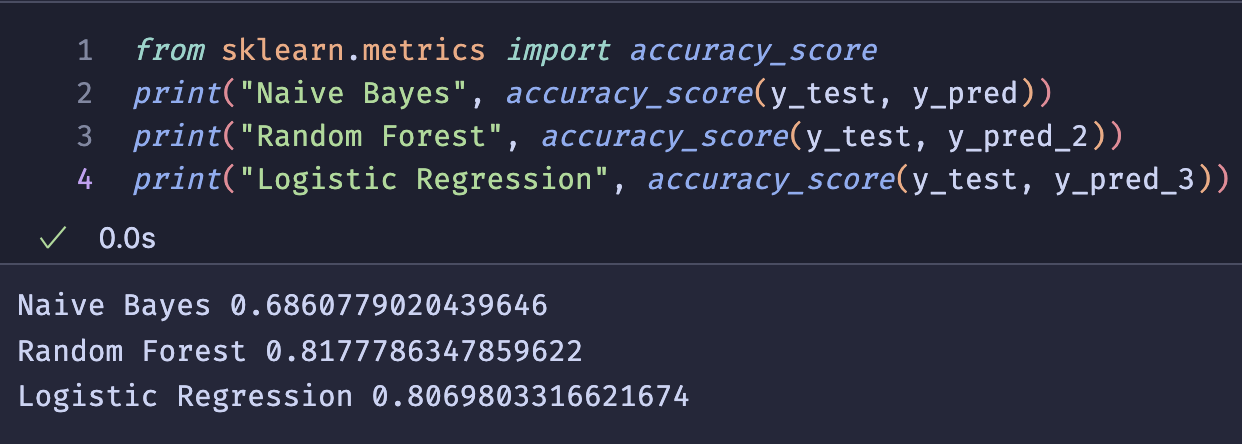
\includegraphics[scale=0.4]{first.png}
\caption{Result showing the baseline accuracy of 3 different algorithms}
\end{figure}
Following this, a cross-validation search was performed on the ranges of hyper parameters for Random Forest since it had the highest
initial accuracy. The ranges chosen are below \-
\begin{figure}[H]
\center
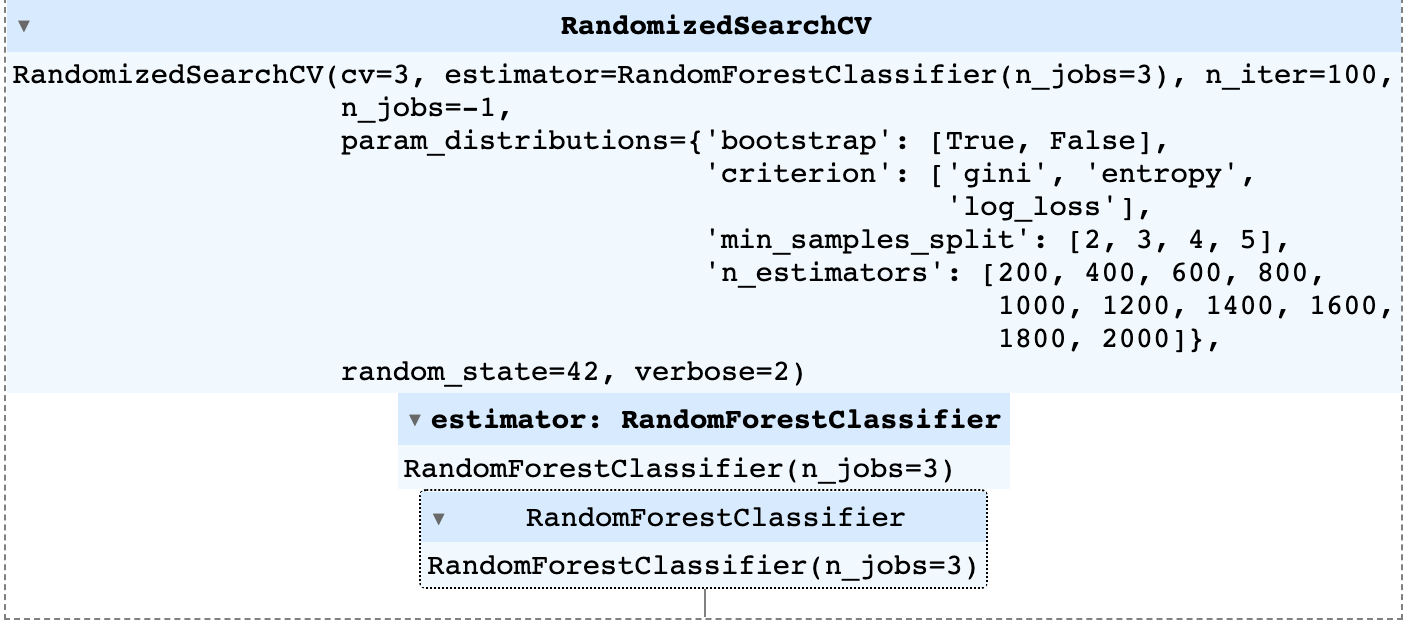
\includegraphics[scale=0.4]{second.png}
\caption{Range of hyperparameter values for CV search}
\end{figure}
We used a 3 fold cross validation over 100 searches making a total of 300 models fit. This provided the following values for the 
hyperparameters -
\begin{figure}[H]
    \center
    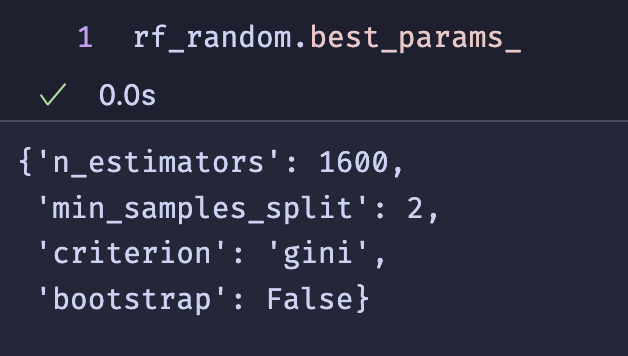
\includegraphics[scale=0.4]{third.png}
    \caption{Range of hyperparameter values for CV search}
\end{figure}
However, many of the ``optimal'' values provided are just the default values of the parameters. Therefore, the increase in accuracy was just 
1\%. The final accuracy is shown below -
\begin{figure}[H]
    \center
    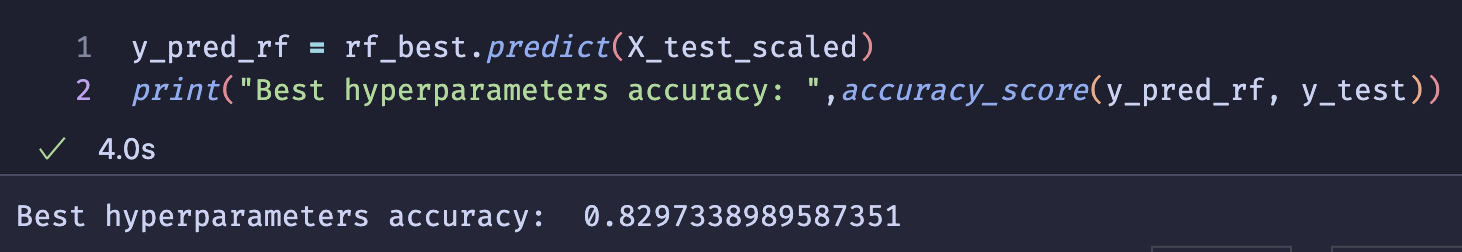
\includegraphics[scale=0.4]{fourth.png}
    \caption{Accuracy with best hyperparameters}
\end{figure}

\end{document}